% **************************************************
%   Wichtig für die verwendung der hsrmreport-Klasse!
%   
%   Die Datei hsrmreport.cls muss in dem selben Ordner sein
%   wie die .tex Datei die diese Klasse verwenden möchte.
%
%   Desweiteren ist die Dokumentenklasse nach aktuellem 
%   noch ohnen Optionen, sprich Zweiseitig, änderung 
%   der Schriftgröße oder ähnliches. Ich werde versuchen 
%   diese Features hinzu zufügen sobald es mir möglich ist. 
%
%   Falls Ihr Probleme, Anregungen oder Verbesserungen habt,
%   könnt ihr mir das gerne mitteilenen.
%
%   Es kann sein das ihr evtl. manche Packete noch installieren 
%   müsst bevor die Klasse Fehlerfrei funktioniert.
%   Meldungen wie "Command terminated with space." können ignoriert werden.
%
%   Ich werde auch eine Übersicht aller Pakete schreiben, die ich verwendet habe.
%      
%
%   E-Mail: timjonas.wechler@student.hs-rm.de
% **************************************************


\documentclass{hsrmreport}
% **************************************************
% Ihr könnte die Angaben der TITELSEITE hier ändern
% **************************************************
\newcommand{\titel}{Versuch 5}
\newcommand{\studiengang}{Angewandte Pyhsik}
\newcommand{\studienrichtung}{}
\newcommand{\dokumentenart}{Praktikumsbericht}
\newcommand{\kurs}{LV:\ Elektronik 1 Praktikum}
\newcommand{\versuchsdurchfuehrung}{16. Januar 2021}

%Falls ihr weniger als vier Studenten seit könnt ihr dies Einträge die zu viel sind einfach löschen. 
%Ein Feature für das angeben der Mat.Nr. ist noch in Arbeit. 
\newcommand{\studentA}{Cassel, Niclas}
\newcommand{\matStudentA}{(1110348)}
\newcommand{\studentB}{Wechler, Tim-Jonas}
\newcommand{\matStudentB}{(1137877)}
\newcommand{\studentC}{}
\newcommand{\matStudentC}{}
\newcommand{\studentD}{}
\newcommand{\matStudentD}{}


% Mit dem Befehl \today wird immer das aktuelle Datum auf der Titelseite ausgebeben.
% Wenn dies nicht erwünscht ist einfach manuell das gewünschte Datum eintragen.
\newcommand{\datum}{\today}



\begin{document}
    % **************************************************
    %
    %   ALLES zwischen hier und dem Begin des Berichts 
    %   nicht ändern, außer ihr wisst was ihr tut ;). 
    %
    % **************************************************

    % Title 
    \frontpage

    %Römischen Seitenzahl
    \pagenumbering{Roman}
    
    %Inhaltsverzeichnis
    \tableofcontents

    %Abbildungsverzeichnis
    \listoffigures

    %Tabellenverzeichnis
    \listoftables

    
    \clearpage

    %Normale Seitenzahlen
    \pagenumbering{arabic}

    %Das seitenLayout mit Kapitel und Unterkapitel im Header jeder Seite des Berichts
    \pagestyle{scrheadings}

    % **************************************************
    %
    % HIER BEGINNT DER BERICHT
    %
    % **************************************************

    
        \chapter{Vorbereitung}
    \section{Aufbau eines Oszilloskop-Tastkopfes}
        Der Tastkopf dient als Verbindung zwischen dem Oszilloskop und der zu messenden Spannung. Es ist auch möglich ein Kabel zu verwenden, jedoch sind dann Widerstand und Kapazität bei der Messung undefiniert. Bei hohen Frequenzen wird dadurch das Messsignal verfälscht. Der Tastkopf kann die Spannung unter bekannten Bedingungen Messen.~\cite{tastkopf_deniz}
        Die Signalverarbeitung eines Tastkopfes kann mit passiven Bauelementen erfolgen oder durch eine aktive Schaltung. Wichtig ist das der Eingangswiderstand eines Tastkopfes möglichst groß und die Einkangskapazität möglichst klein ist, damit das Signal unverfälscht weitergegeben wird. Dabei gibt es viele verschiedene Tastköpfe mit eigenen Eigenschaften. Im Folgenden sind diese mit ihrem Aufbau aufgelistet.~\cite{tastkopf_wiki}

        \begin{enumerate}

        \item Standard-Tastkopf
            \begin{figure}[h!]
                \centering
                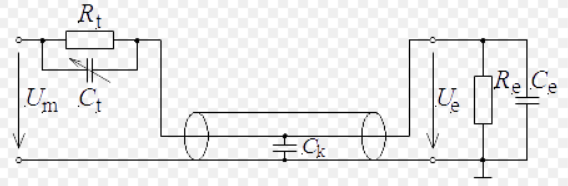
\includegraphics[]{111.PNG}
                \caption{Aufbau eines Standart Tastkopfes~\cite{tastkopf_standard}}
            \end{figure}

        \item Transmissions-Line-Tastkopf
            \begin{figure}[h!]
                \centering
                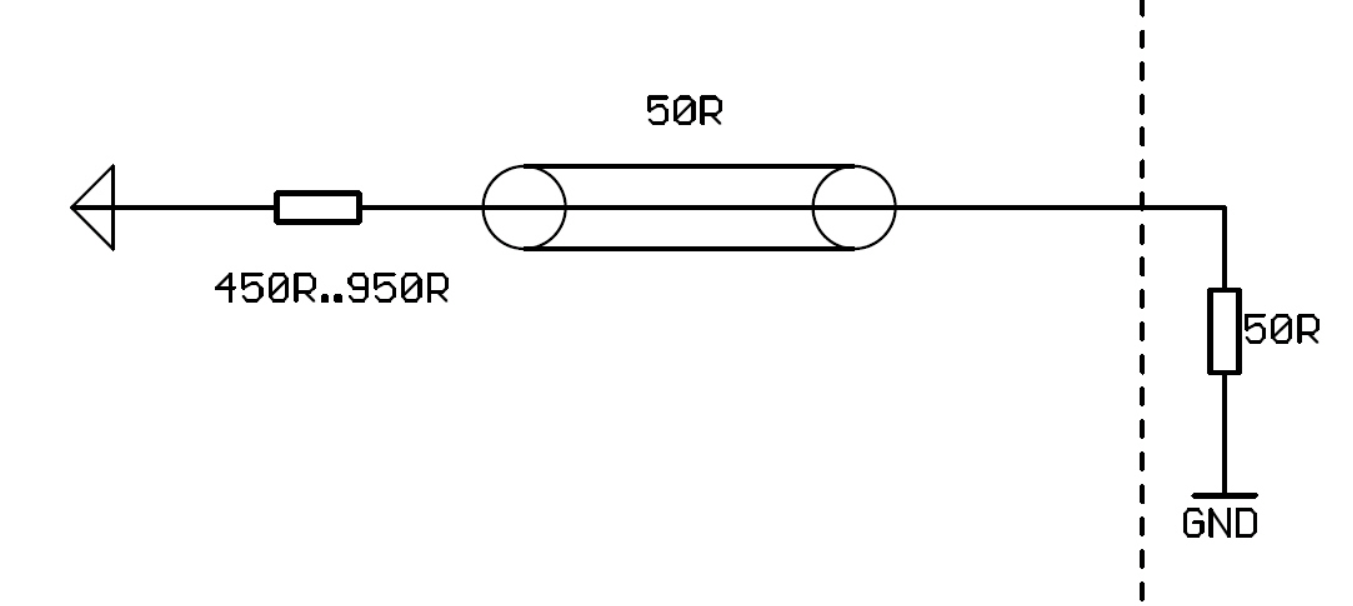
\includegraphics[width=0.5\linewidth]{112.PNG}
                \caption{Aufbau eines Transmission-Line-Tastkopfes~\cite{transmission_line_probe}}
            \end{figure}
        \newpage
        \item Aktiver Tastkopf
            \begin{figure}[h!]
                \centering
                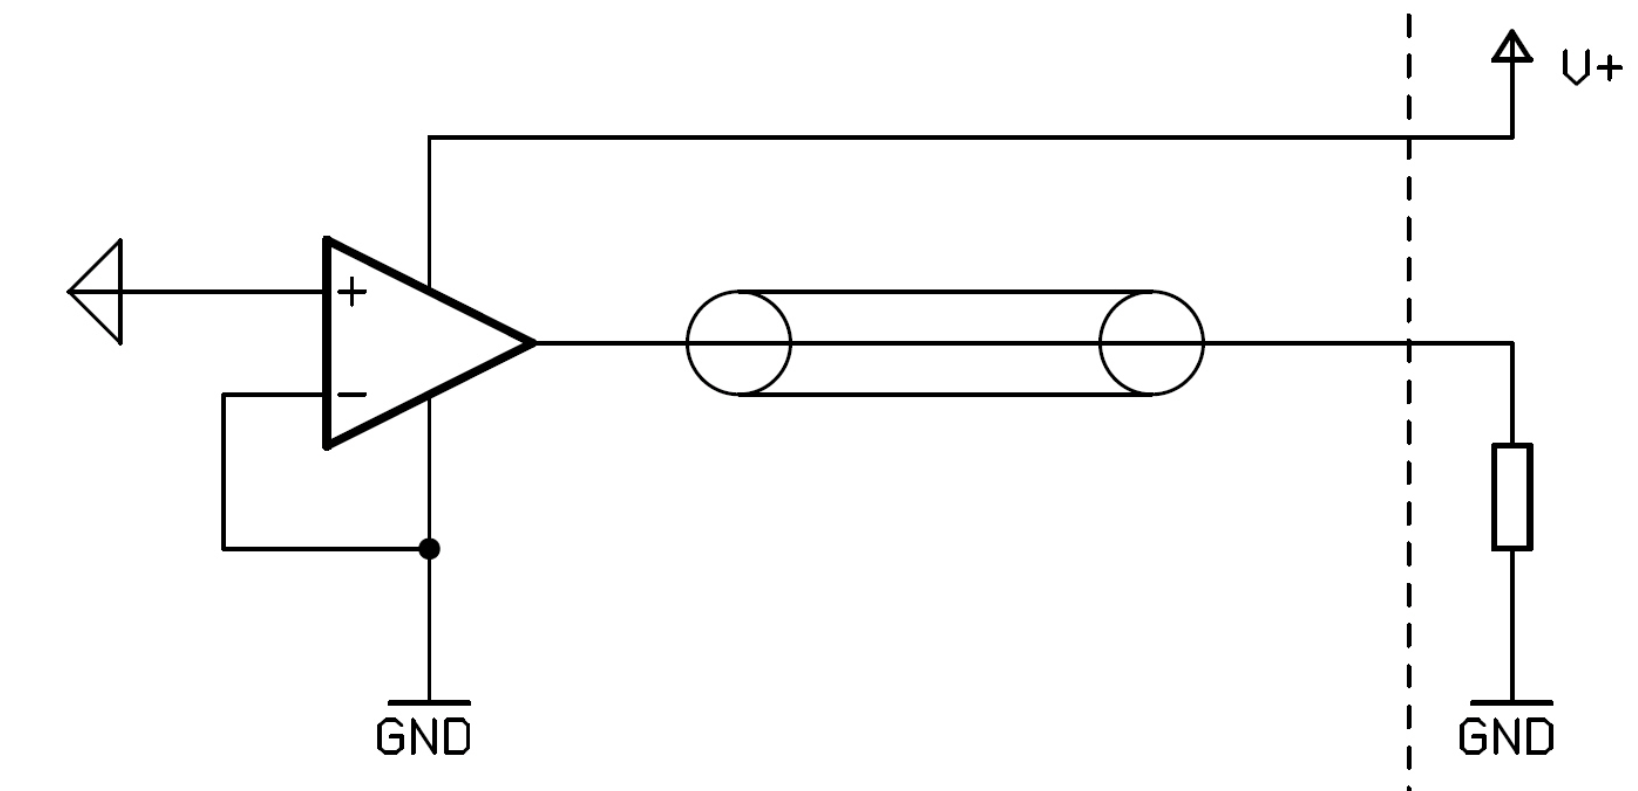
\includegraphics[width=0.5\linewidth]{113.PNG}
                \caption{Aufbau eines aktiven Tastkopfes~\cite{active_probe}}
            \end{figure}

        \item Differentieller Tastkopf
            \begin{figure}[h!]
                \centering
                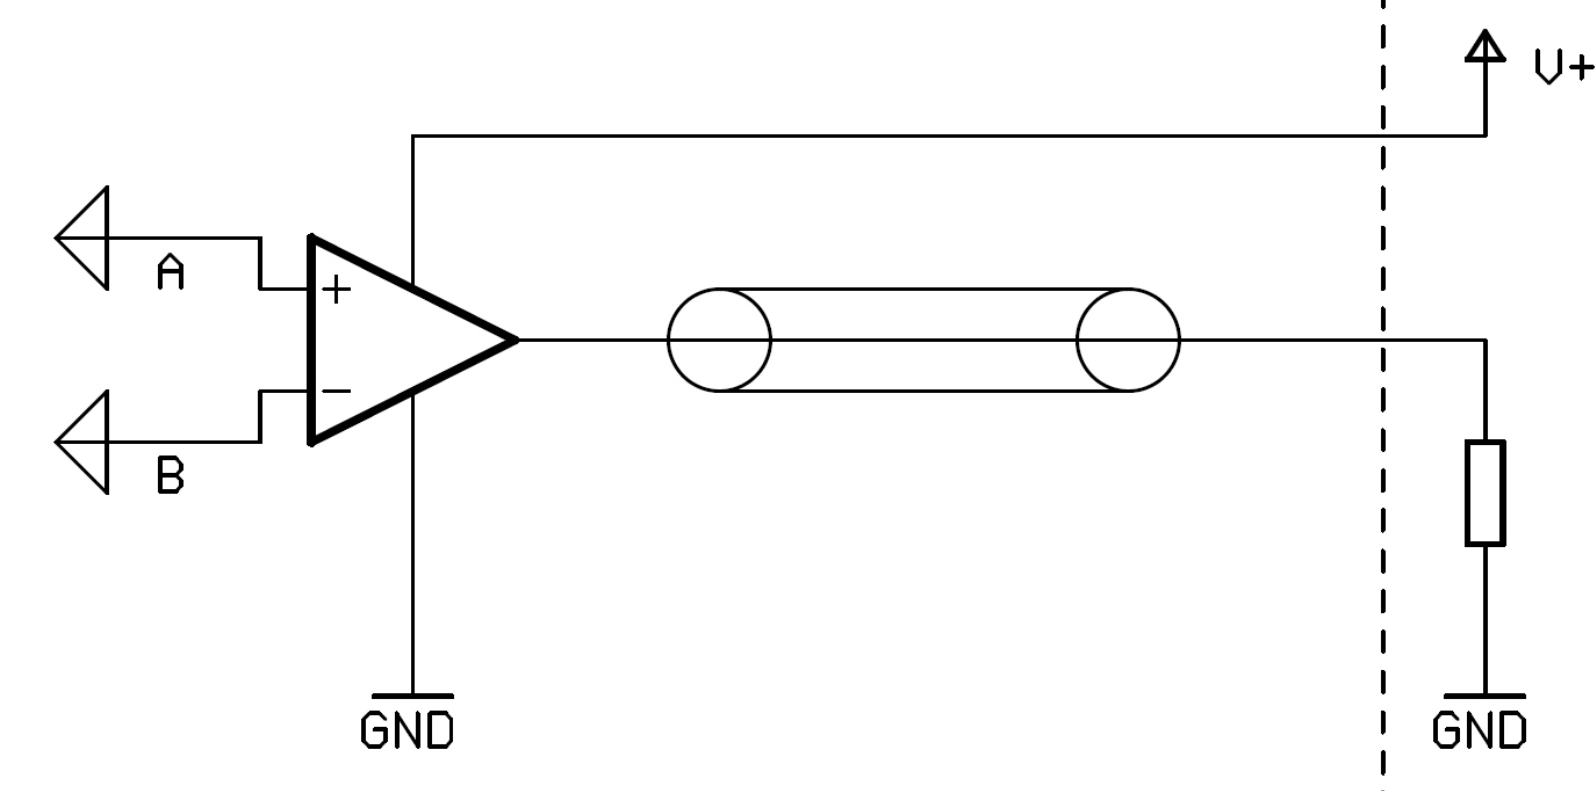
\includegraphics[width=0.5\linewidth]{114.PNG}
                \caption{Aufbau eines differentiellen Tastkopfes~\cite{differential_probe}}
            \end{figure}

        \end{enumerate}

        \begin{table}[h!]
            \centering
            \caption{Begriffserklärung für die einzelnen Buchstaben in den Abbildungen}
            \begin{tabular}{|c|c|}
                \hline
                $R_t$ & Tastkopfwiderstand\\ \hline \hline
                $C_t$ & Tastkopfkapazität \\ \hline
                $U_m$ & Spannungsmessung\\ \hline
                $C_K$ & Kabelkapazität\\ \hline
                $U_e$ & Eingangsspannung\\ \hline
                $R_e$ & Eingangswiderstand\\ \hline
                $C_e$ & Eingangskapazität\\ \hline
                Zahl mit R & Widerstand mit Zahlenwert \\ \hline
                GND & Ground (zu Erde)\\ \hline
                V & Spannung\\ \hline
            \end{tabular}
        \end{table}


        \input{content/versuchsdurchführung.tex}
        \chapter{Aufgaben}
Bei den Aufgaben werden mit LTSpice Schaltungen zusammengestellt, welche dann praktisch im Labor nachgebaut werden können. In den folgenden Aufgaben werden verschiedene Schaltungen wie Signalquellen, Spannungsteiler und Potentiometer zusammengestellt. 

\section{Signalquellen}
Hier ist der Aufbau einer einfachen Signalquelle zu sehen, welche eine Spannung von 1V besitzt.
\begin{figure}[h!]
\centering
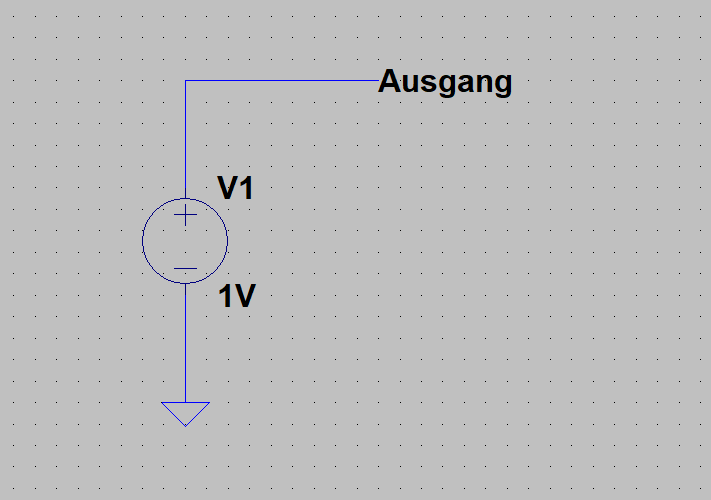
\includegraphics[scale=1]{21.PNG}
\caption{Darstellung einer Signalquelle in LTSpice}
\label{fig: Signalquelle}
\end{figure}
\newpage
Im Folgenden werden mit der Schaltung \fref{fig: Signalquelle}, verschieden Kurvenformen dargestellt und mit den jeweiligen Werten in LTSpice simuliert:



\subsection{Gleichspannungsquelle}
Folgender LTSpice Simulation und Graph wird durch eine Gleichspannungsquelle erzeugt.
\begin{figure}[ht!]
\centering
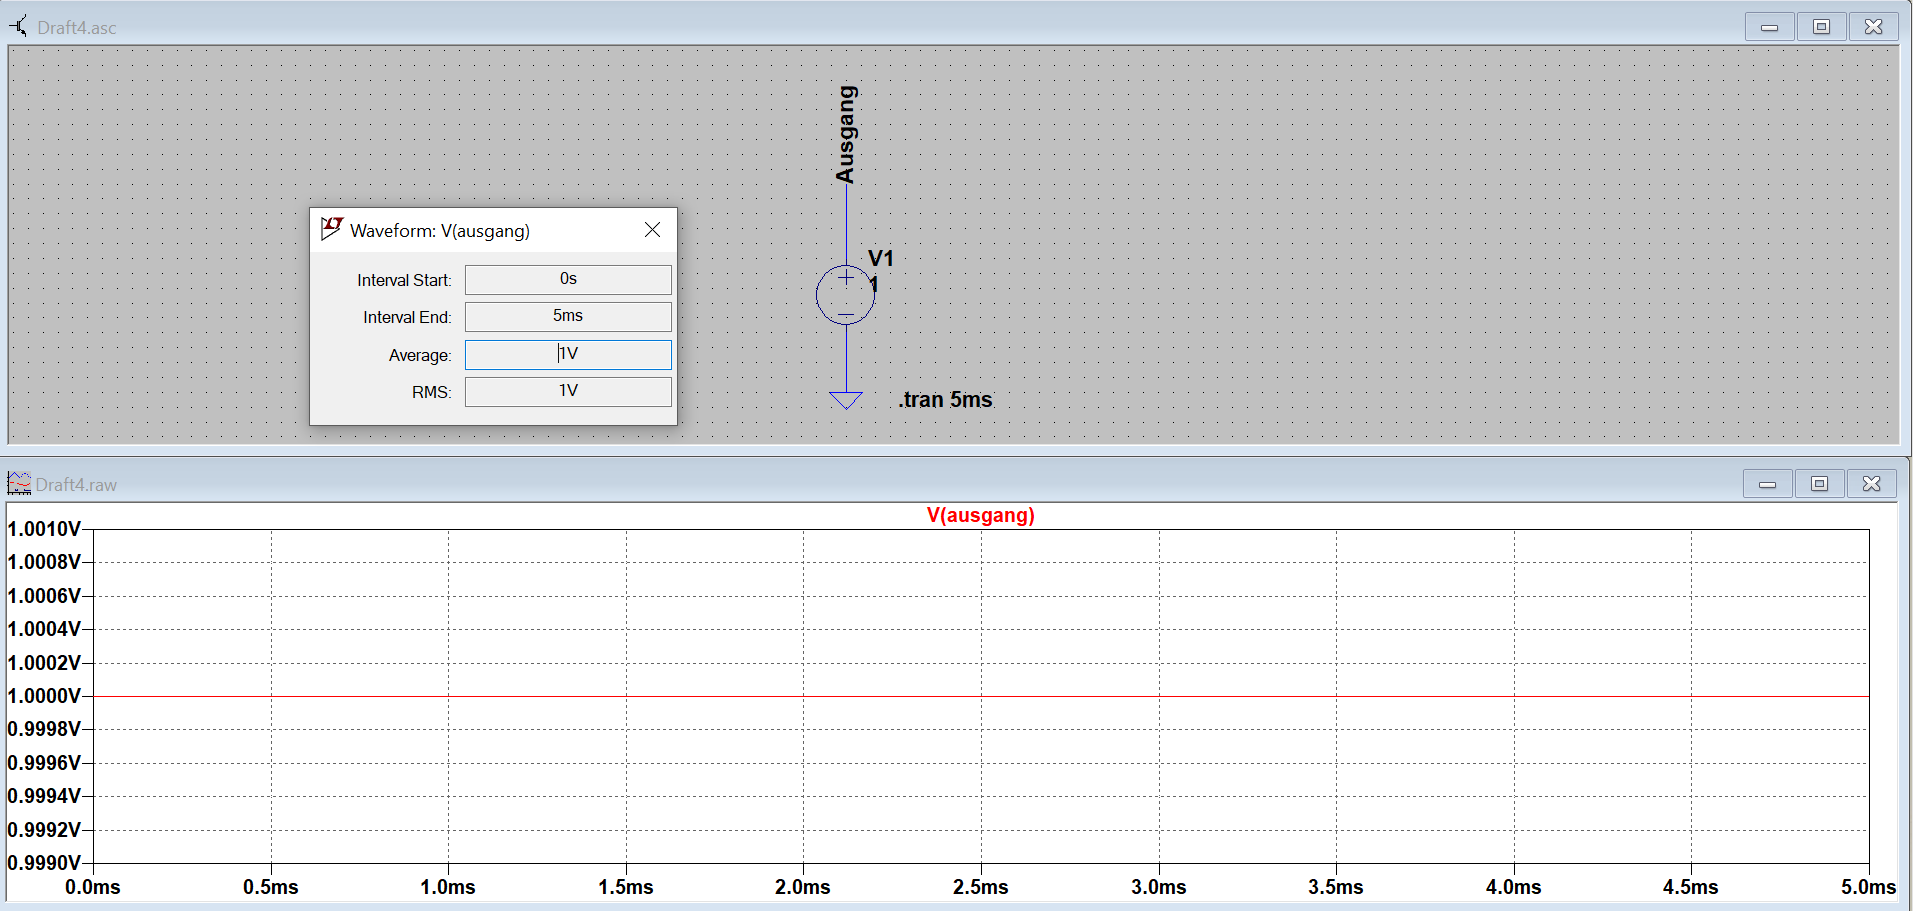
\includegraphics[scale=0.5]{211.PNG}
\caption{Gleichspannungsquelle $U=1V$}
\end{figure}

\subsection{Signussignal}
Um bei der folgenden Simulation ein richtiges Signal heraus zu bekommen, muss die $Periode(T)=1ms$ in die Frequenz f umgerechnet werden.
\begin{equation}
f=\frac{1}{T}=\frac{1}{10^{-3}}=1000Hz
\end{equation}
Folgender LTSpice Simulation und Graph wird durch die Werte erzeugt.
\begin{figure}[h!]
\centering
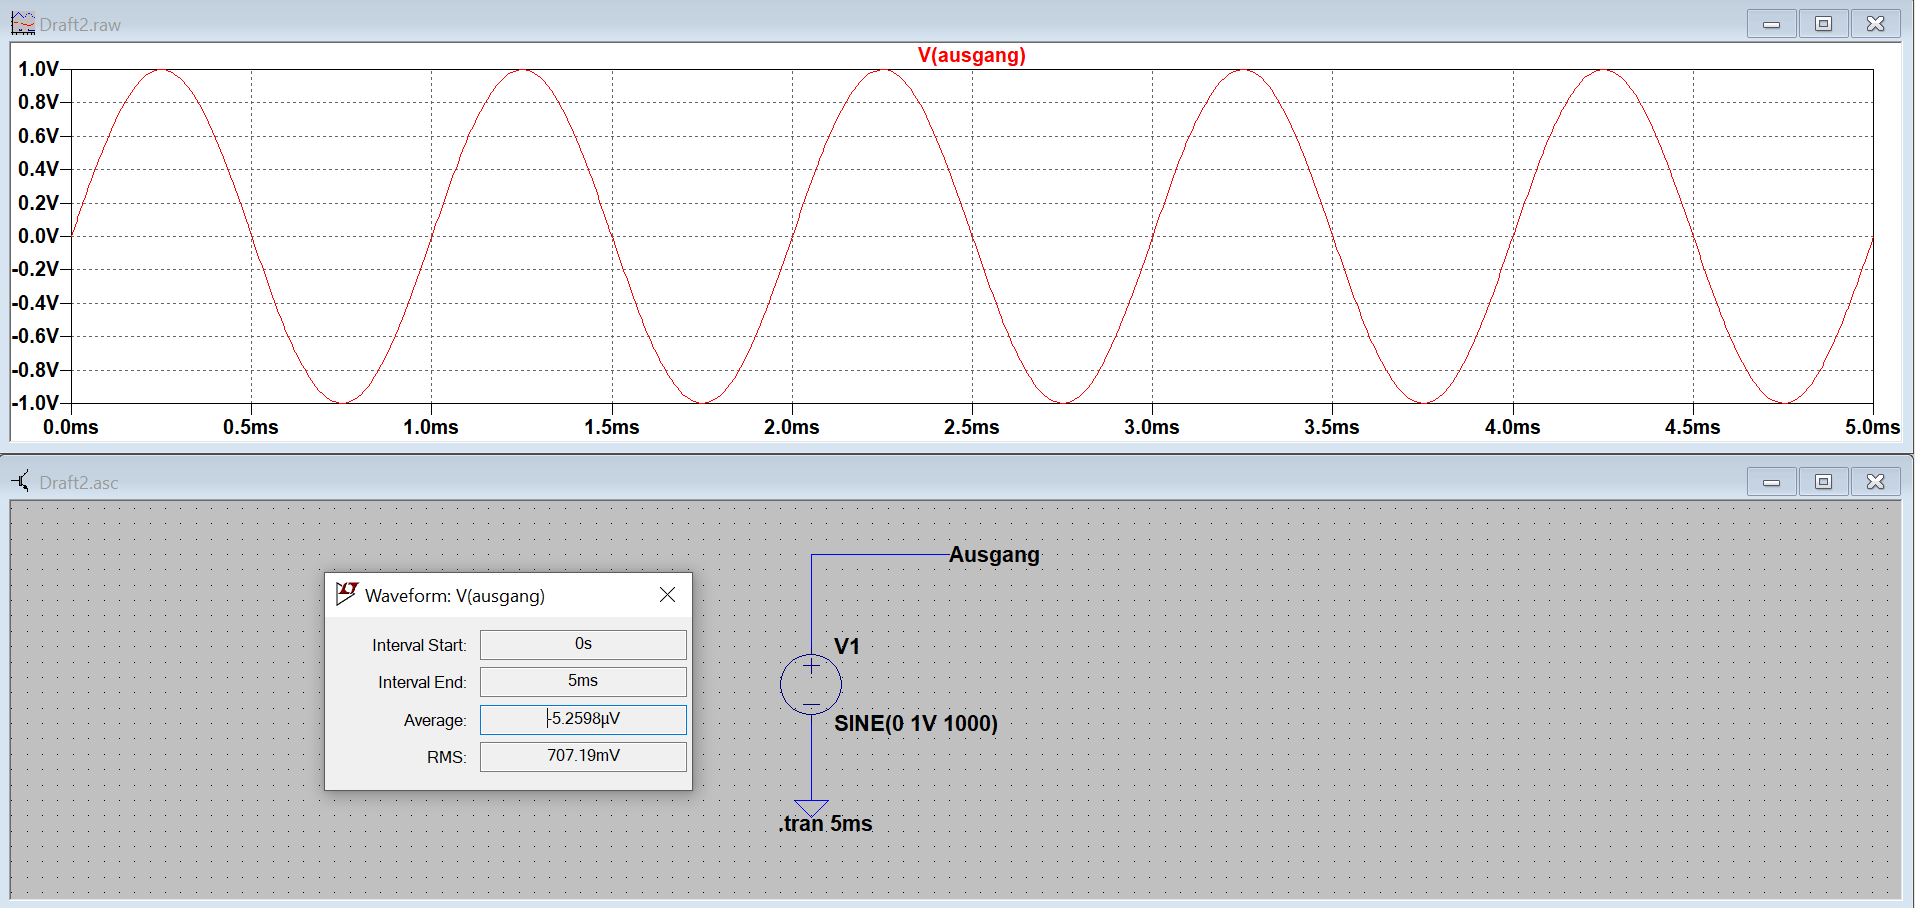
\includegraphics[scale=0.5]{212.PNG}
\caption{Sinussignal mit $\^{U}=1V$ und $T=1ms$}
\label{fig: Sinussignal}
\end{figure}
\newpage

\subsection{Symmetrisches Rechtecksignal}
Zum Darstellen eines symmetrischen Recktecksignals wird der $T_{rise}$ und $T_{fall}$ Wert angepasst. Dieser liegt in der Simulation bei jeweils 1ns. Die Spannungsquelle wird in den Pulse-Mode gestellt und die Werte für $\^{U}$,$T_{on}$ und f eingetragen \fref{fig: symRechtecksignal}. Dabei ergibt sich folgende LTSpice Simulation und Graph. 
\begin{figure}[ht!]
\centering
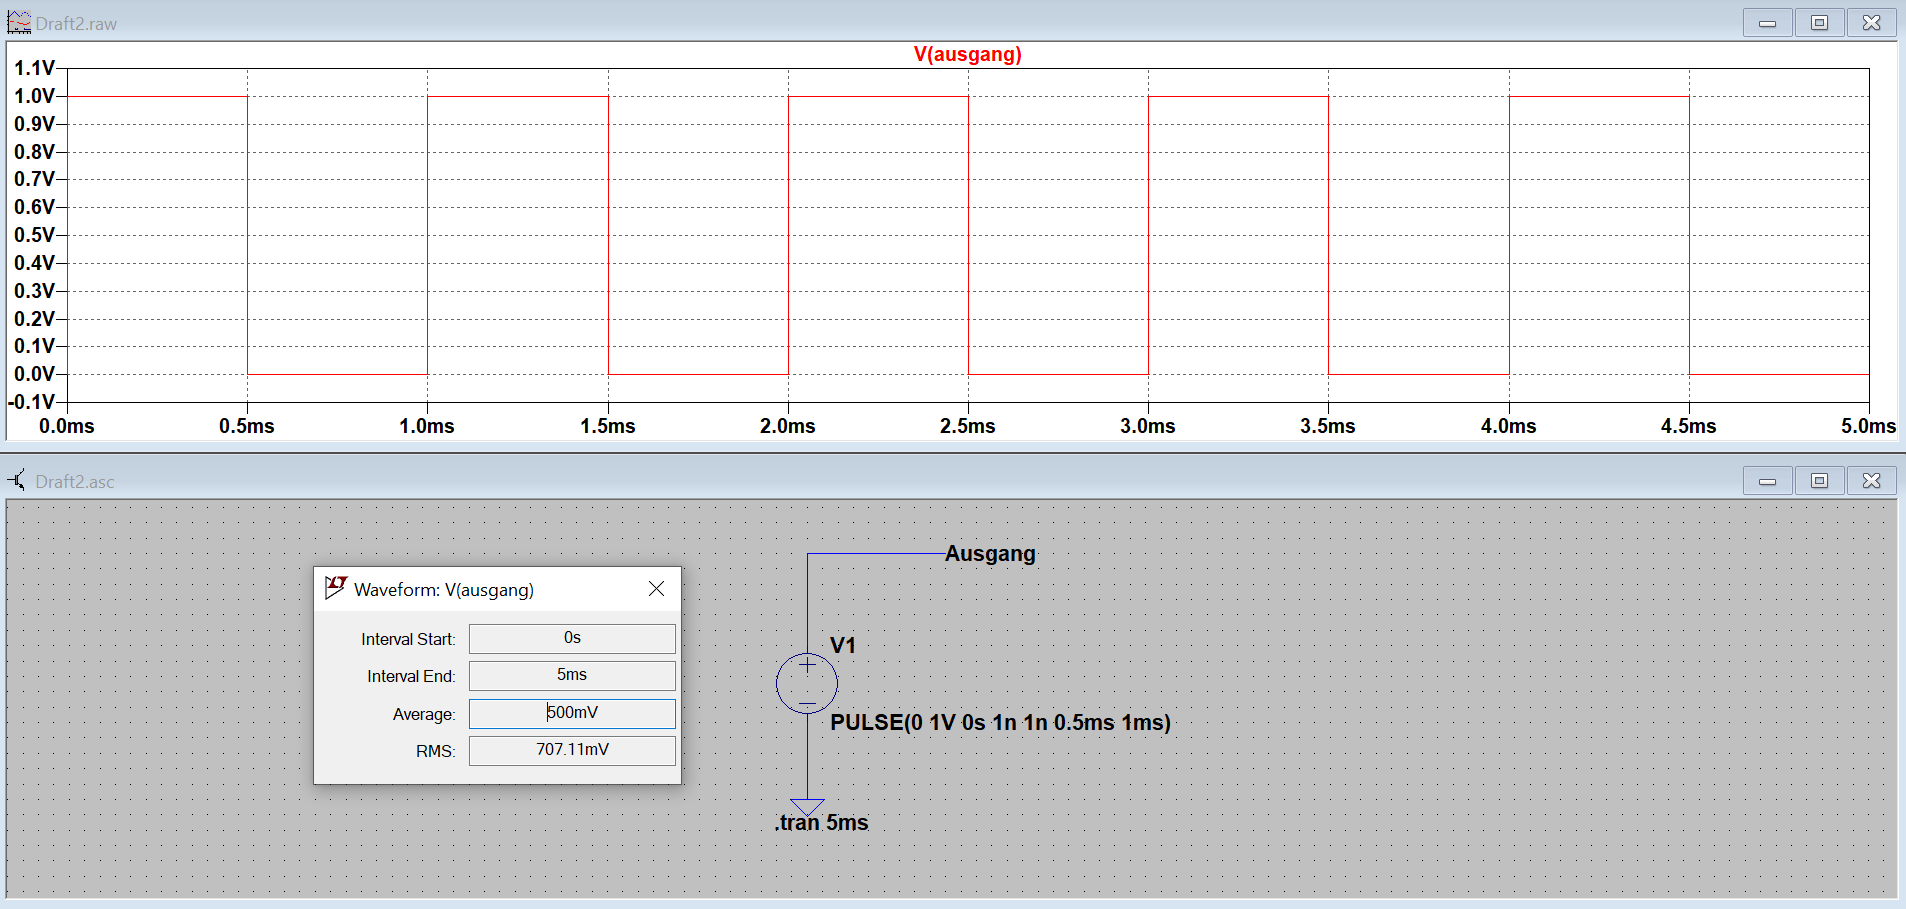
\includegraphics[scale=0.5]{213.PNG}
\caption{Symmetrisches Rechtecksignal mit $\^{U}=1V$, $T_{on}=0,5 ms$ und $f=1ms$}
\label{fig: symRechtecksignal}
\end{figure}

\subsection{Unsymmetrisches Rechtecksignal}
Zum Darstellen eines unsymmetrischen Recktecksignals wird ebenfalls der $T_{rise}$ und $T_{fall}$ Wert angepasst. Der liegt bei dieser Simulation bei jeweils 1ns. Durch eintragen der restlichen Werte \fref{fig: unsymRechtecksignal}, ergibt sich folgende LTSpice Simulation und Graph.
\begin{figure}[ht!]
\centering
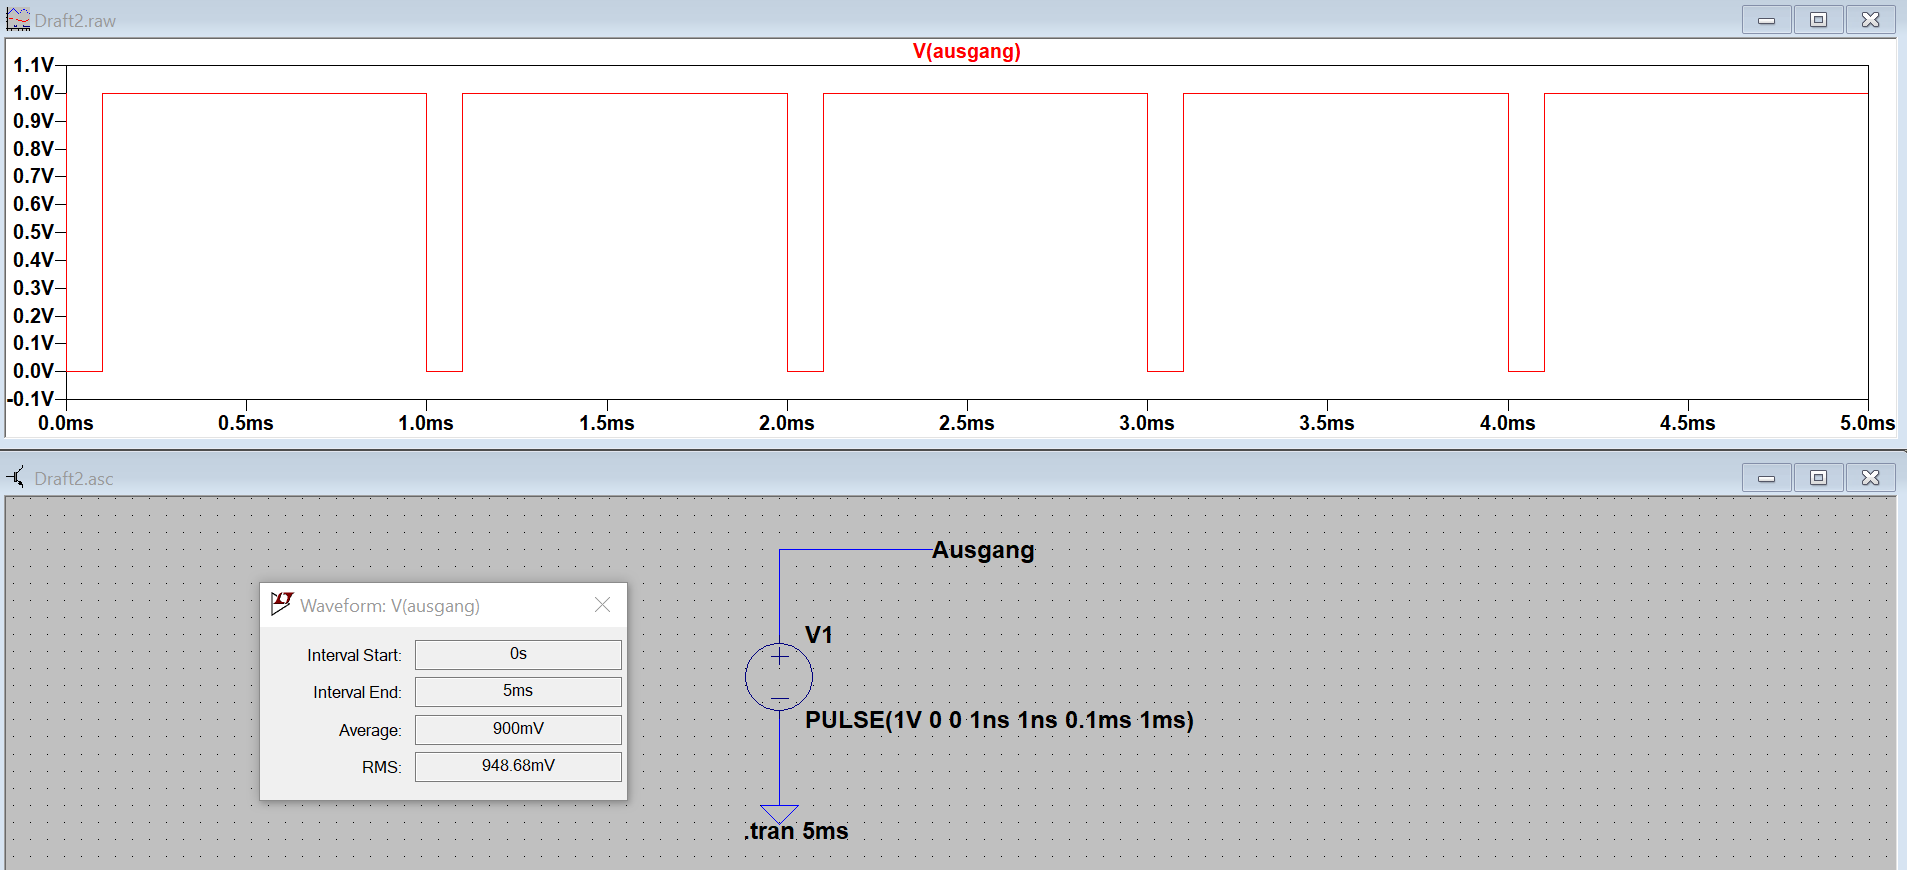
\includegraphics[scale=0.5]{214.PNG}
\caption{Unsymmetrisches Rechtecksignal mit $\^{U}=1V$, $T_{on}=0,1 ms$ und $f=1ms$}
\label{fig: unsymRechtecksignal}
\end{figure}

\subsection{Dreiecksignal}
Damit bei der Simulation mit LTSpice ein Dreiecksignal herauskommt, werden die Werte für $T_{rise}$, $T_{fall}$ und $T_{on}$ angepasst. 
$$T_{rise}=0.5ms$$
$$T_{fall}=0.5ms$$
$$T_{on}=0ms$$
Durch das einfügen der restlichen Werte \fref{fig: Dreiecksignal}, ergibt sich folgende LTSpice Simulation und Graph.
\begin{figure}[ht!]
\centering
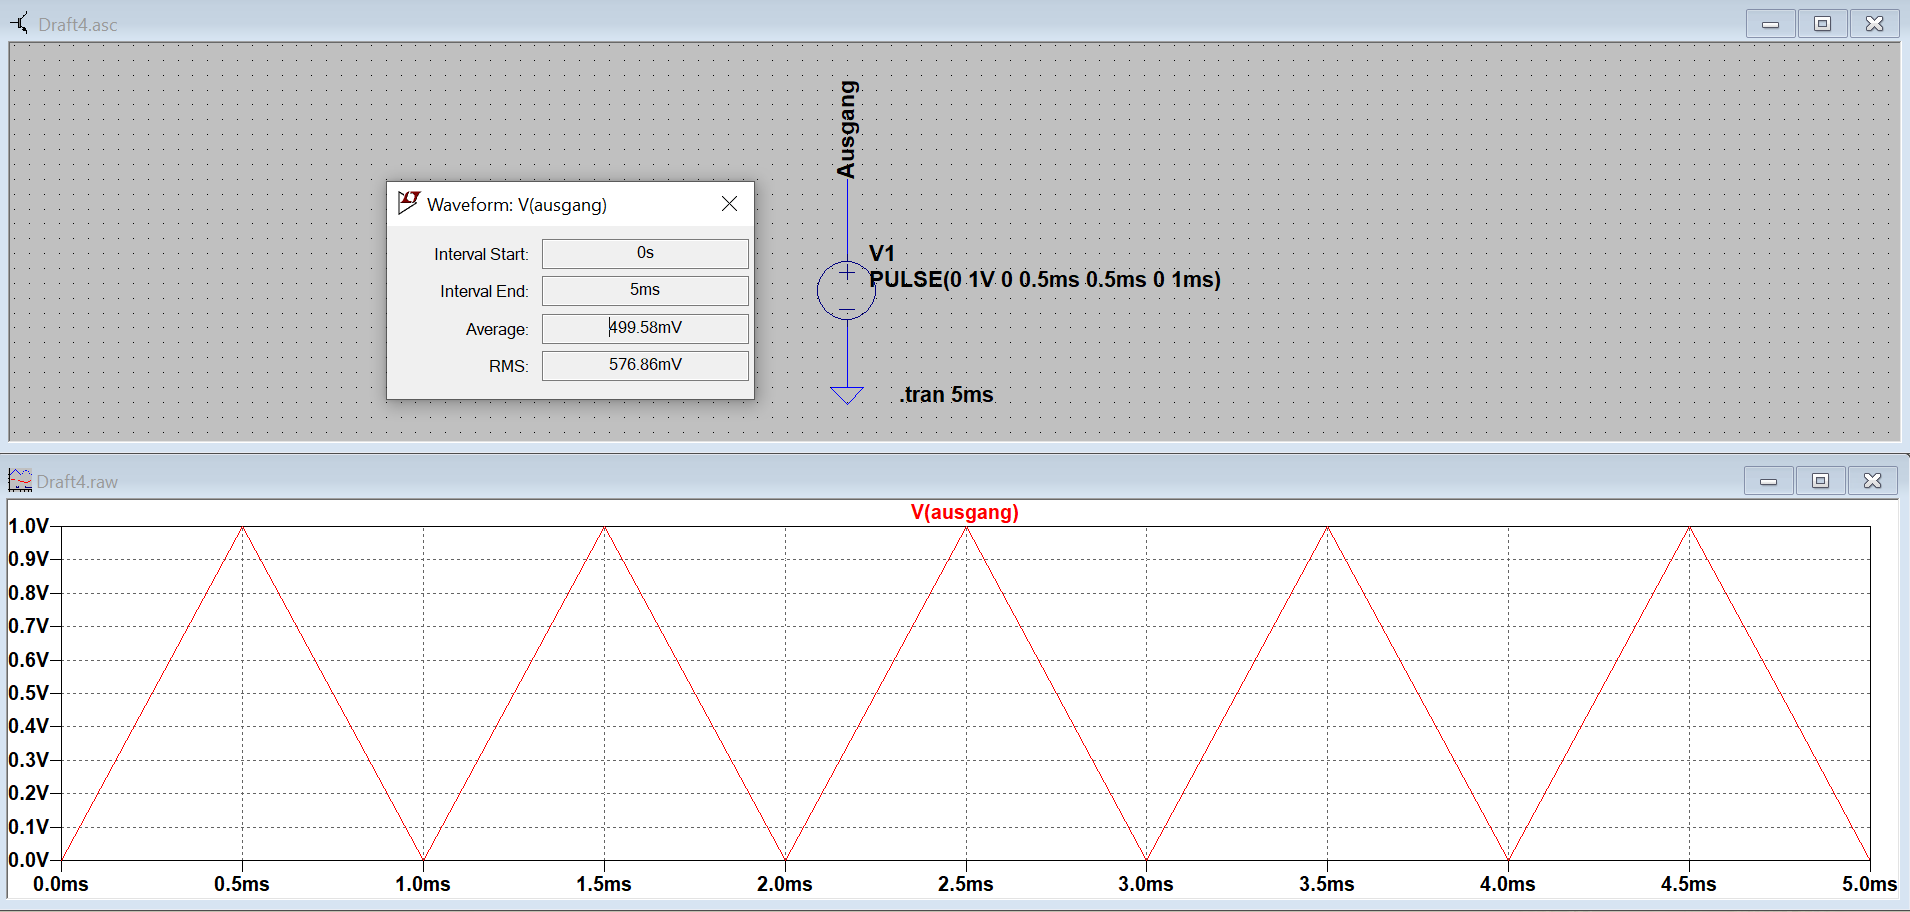
\includegraphics[scale=0.5]{215.PNG}
\caption{Dreiecksignal mit $\^{U}=1V$, $T=1ms$ }
\label{fig: Dreiecksignal}
\end{figure}
\newpage
\subsection{Sägezahnsignal}
Damit bei der Simulation mit LTSpice ein Dreiecksignal herauskommt, werden die Werte für $T_{rise}$, $T_{fall}$ und $T_{on}$ angepasst. 
$$T_{rise}=0.5ms$$
$$T_{fall}=1ns$$
$$T_{on}=0ms$$
Durch das einfügen der restlichen Werte \fref{fig: Sägezahnsignal}, ergibt sich folgende LTSpice Simulation und Graph.

\begin{figure}[ht!]
\centering
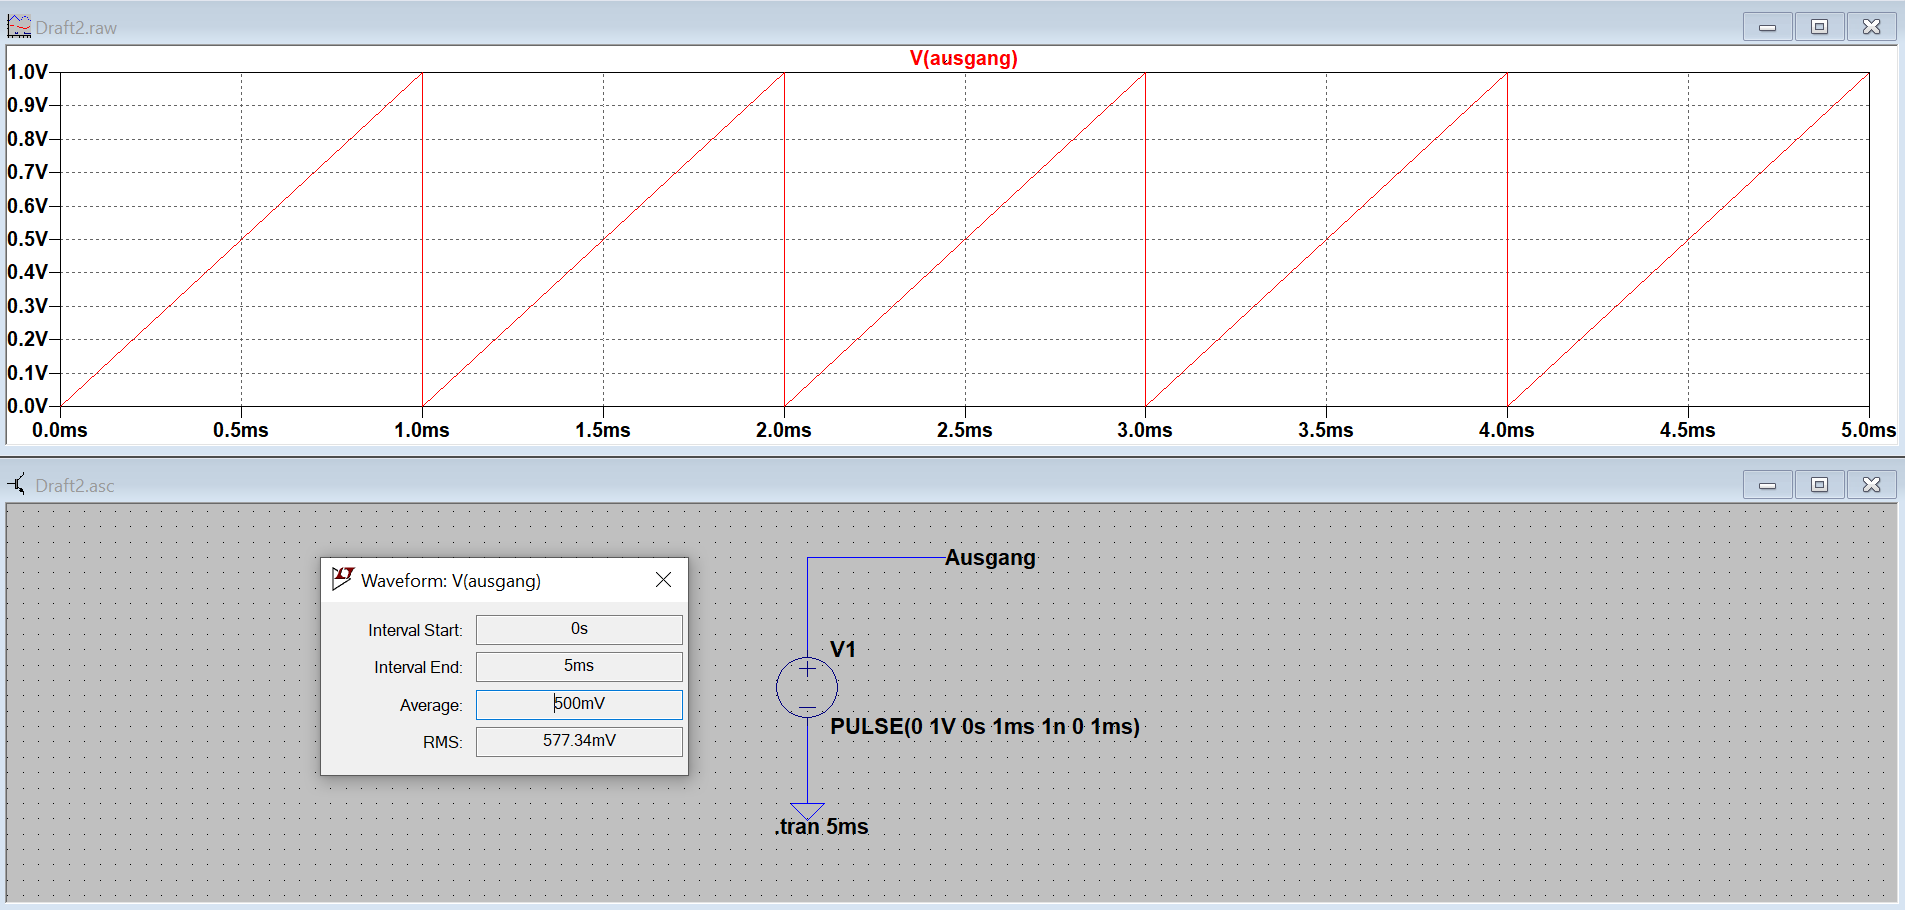
\includegraphics[scale=0.5]{216.PNG}
\caption{Sägezahnsignal mit $\^{U}=1V$, $T=1ms$}
\label{fig: Sägezahnsignal}
\end{figure}



Die von Hand ermittelten Effektivwerte (siehe Abschnitt 1.3) werden im Folgenden mit den Werten aus der Simulation verglichen. Die simulierten Effektivwerte sind auf den einzelnen Abbildungen \ref{fig: Signalquelle} bis \ref{fig: Sägezahnsignal} in den kleinen Kästchen unter RMS zu finden.
\begin{table}[ht!]
\centering
\caption{Wertetabelle für die Effektivwerte}
\label{fig: Effektivwerte}
\begin{tabular}{|c|c|c|} \hline
Signal & simulierte Effektivwerte & berechnete Effektiverte\\ \hline
Gleischspannungsquelle & 1V & 1V\\ \hline
Sinussignal & 707,19mV & 707mV\\ \hline
Symmetrisches Rechtecksignal & 707,11mV & 1V\\ \hline
Unsymmetrisches Rechtecksignal & 948,68mV & 1V\\ \hline
Dreiecksignal & 576,86mV & 578mV\\ \hline
Sägezahnsignal & 577,34mV & 578mV\\ \hline

\end{tabular}
\end{table}

Den Wert für das Sinussignal wurde in 1.3.1 Formel (1.9) berechnet. Der Wert für die Rechtecksignale sind in 1.3.2 Formel (1.17) und für die Dreiecksignale  in 1.3.3 Formel (1.26) zu finden. In Tab. \ref{fig: Effektivwerte} sind diese nochmal nebeneinander gestellt. Beim Vergleichen der Effektivwerte durch Berechnen und durch die Simulation ist direkt zu sehen, dass es dort kleine Unterschiede gibt. Bei dem Sinussignal und dem Dreiecksignal sind die Werte annäherungsweise gleich. Jedoch gibt es bei den Rechtecksignalen Unterschiede zwischen den Effektivwerten. Der des unsymmetrischen Dreiecksignals ist noch annäherungsweise an den errechneten 1V dran, der Effektivwert des symmetrischen Rechtecksignals hat jedoch einen Unterschied von fast 300mV. Dieser Wert passt eher zu dem berechneten Effektivwert des Sinussignals.

\newpage


\section{Spannungsteiler}
\subsection{Unbelasteter Spannungsteiler}
\begin{figure}[h!]
\centering
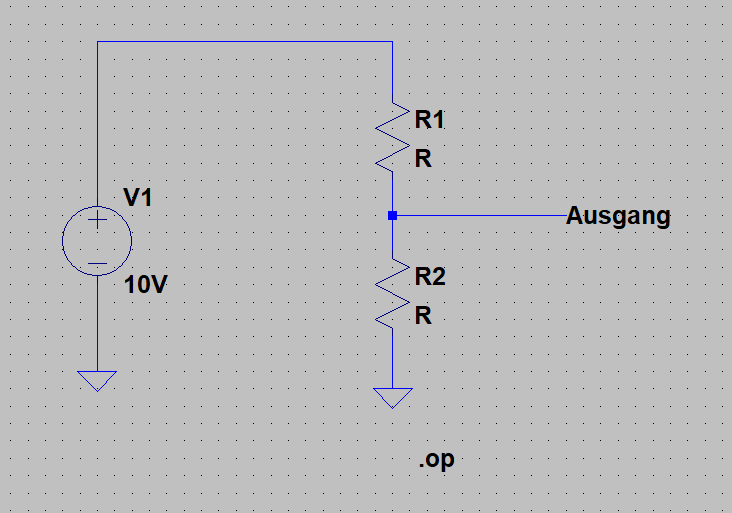
\includegraphics[scale=1]{221.PNG}
\caption{Unbelasteter Spannungsteiler}
\label{fig: Unbelasteter Spannungsteiler}
\end{figure}
Beim unbelasteten Spannungsteiler \fref{fig: Unbelasteter Spannungsteiler} werden jetzt die einzelnen Werte für $R_1$ und $R_2$ verändert und in die Schaltung eingegeben.

\begin{table}[h!]
\centering
\caption{Wertetabelle für den unbelasteten Spannungsteiler }
\label{fig: unbelasteter Spannungsteiler}
\begin{tabular}{|c|c|c|c|} \hline
$R_1$ in $\Omega$ & $R_2$ in $\Omega$ & $V_{aus}$ Simulation in V & $V_{aus}$ Spannungsteilerformel in V\\ \hline
$4,7k$ & $2,2k$ & 3,18841 & 3,18841\\ \hline
$47k$ & $22k$ & 3,18841 & 3,18841\\ \hline
$470k$ & $220k$ & 3,18841 & 3,18841\\ \hline
$4,7M$ & $2,2M$ & 3,18841 & 3,18841\\ \hline
$47M$ & $22M$ & 3,18841 & 3,18841\\ \hline

\end{tabular}
\end{table}

Mit der Spannungsteilerformel 
\begin{equation}
U_{aus}=U_{ges}\cdot \frac{R_2}{R_1+R_2}
\end{equation}
wird die Spannung am Ausgang von Hand berechnet. Dabei ist $U_{ges}=10V$, die Werte für $R_1$ und $R_2$ sind aus der Tabelle \ref{fig: unbelasteter Spannungsteiler} ablesbar.
Die Ergebnisse der Simulation und die Ergebnisse aus der Spannungsteilerformel sind identisch. Desweiteren sind die Ergebnisse für die verschiedenen Werte von $R_1$ und $R_2$ gleich, da diese Vielfache voneinander sind und sich somit die erhöhten Werte ausgleichen.

\subsection{Belasteter Spannungsteiler}
Der belastete Spannungsteiler ist wie der unbelastete Spannungsteiler aufgebaut, jedoch wird an den Ausgang ein Innenwiderstand von $R_3=10M\Omega$ dazugeschaltet. Dies ist in Abb.\ref{fig: bel.Spannungsteiler} veranschaulicht.
\begin{figure}[h!]
\centering
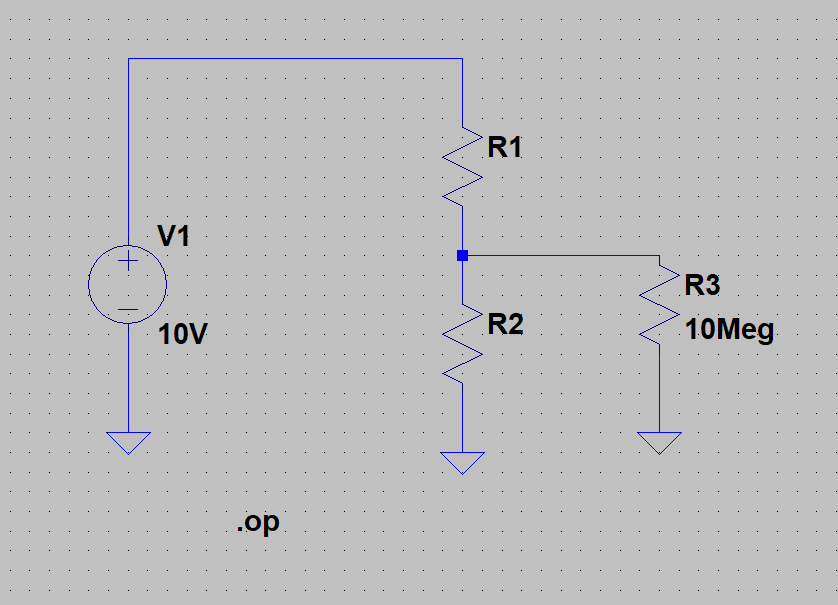
\includegraphics[scale=1]{222.PNG}
\caption{Belasteter Spannungsteiler}
\label{fig: bel.Spannungsteiler}
\end{figure}

\begin{table}[h!]
\centering
\caption{Wertetabelle für den unbelasteten Spannungsteiler }
\label{fig: belasteter Spannungsteiler}
\begin{tabular}{|c|c|c|} \hline
$R_1$ in $\Omega$ & $R_2$ in $\Omega$ & $V_{aus}$ Simulation in V \\ \hline
$4,7k$ & $2,2k$ & 3.18793\\ \hline
$47k$ & $22k$ & 3.18363\\ \hline
$470k$ & $220k$ & 3.14133\\ \hline
$4,7M$ & $2,2M$ & 2.77288\\ \hline
$47M$ & $22M$ & 1.2761\\ \hline

\end{tabular}
\end{table}

Beim Vergleichen der Ausgangsspannung $V_{aus}$ der Simulation (siehe Tab.~\ref{fig: belasteter Spannungsteiler} und~\ref{fig: unbelasteter Spannungsteiler})fällt auf das die Werte voneinander abweichen. Das liegt daran, das ein nicht variabler Widerstand $R_3=10M\Omega$ (Innenwiderstand des Voltmeters) parallel zu $R_2$ dazugeschaltet ist. Da dieser immer den gleichen Wert besitzt, jedoch die Werte für $R_1$ und $R_2$ steigen, verändert sich auch die Spannung am Ausgang. Dies  ist auch an der Formel für einen belasteten Spannungsteiler zu sehen.
\begin{equation}
U_{aus}=U_{ges}\cdot \frac{R_2||R_3}{R_1+(R_2||R_3)}
\end{equation}
Hier wird der Widerstand $R_3$ parallel zu $R_2$ geschaltet und  mit dem festen Wert für $R_3$ gerechnet. Dadurch sinkt die Spannung bei höheren Widerstandswerten von $R_1$ und $R_2$.

\section{Potentiometer}
\begin{figure}[h!]
\centering
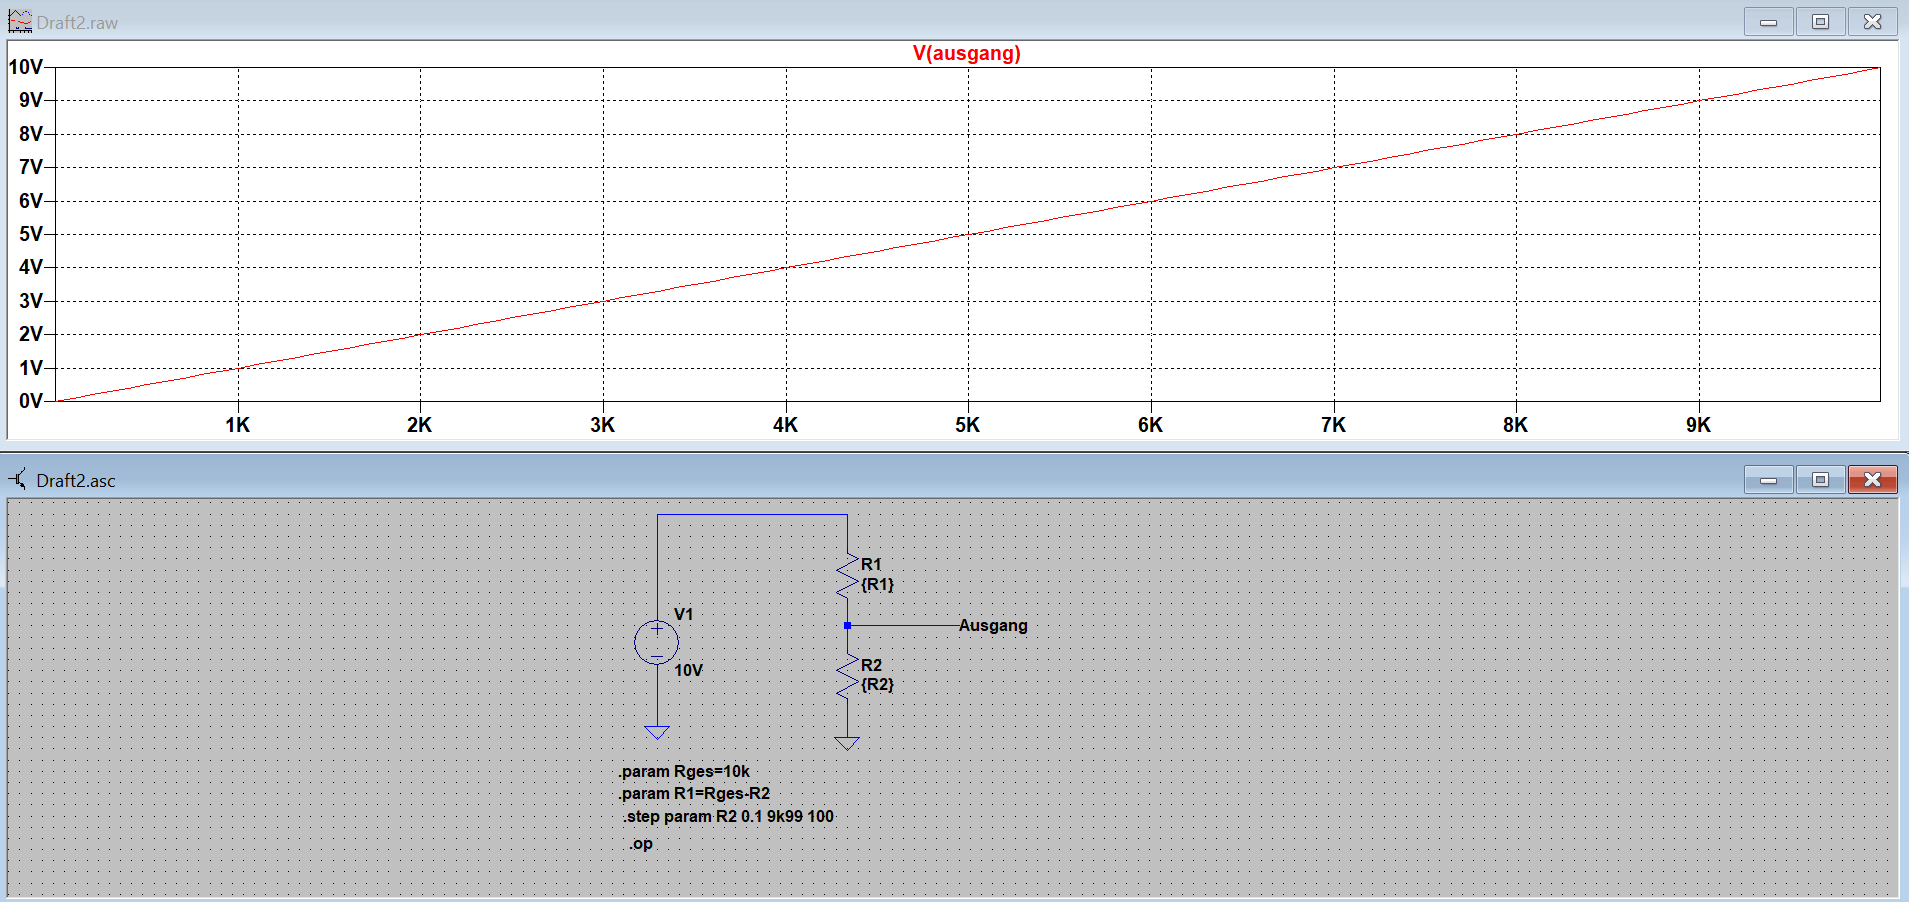
\includegraphics[scale=0.5]{23.PNG}
\caption{Darstellung eines Potentiometers}
\label{fig: Potentiometer}
\end{figure}

Die Schaltung in Abb.~\ref{fig: Potentiometer} sieht aus wie die Abb.~\ref{fig: Unbelasteter Spannungsteiler} eines unbelasteten Spannungsteilers. Jedoch ist beim Potentiometer der Widerstand $R_1$ vom Widerstand $R_2$ abhängig.
\begin{equation}
R_1=R_{ges}-R_2
\end{equation}
Die Werte von $R_2$ ändern sich dabei in $100\Omega$ Schritten im Intervall von $0.1\Omega$ bis $9k99\Omega$, unter der Bedingung:
$$0\Omega \leq R_2\leq R_{ges}$$
Die Simulation beginnt mit $0.1\Omega$ und endet mit $9k99\Omega$ damit $R_1$ nicht $0\Omega$ wird.\\
Im Graphen \fref{fig: Potentiometer} ist zu sehen, das mit steigendem $R_2$ auch die Ausgangsspannung $V_{aus}$ steigt.








        
    \section{Frequenzgang der Gleichtaktverstärkung}
        Um nun die Gleichtaktverstärkung zu simulieren wird die Spannung von \(U_{V3}\) auf \SI{0}{\V} und die Spannung \(U_{V4}\) auf \SI{1}{\V} gesetzt.
        Somit sorgt dafür das \textbf{Eingang 1} und \textbf{Eingang 2} jeweils mit der gleichen Spannung versorgt werden. 
        \begin{figure}[ht!]
            \centering
            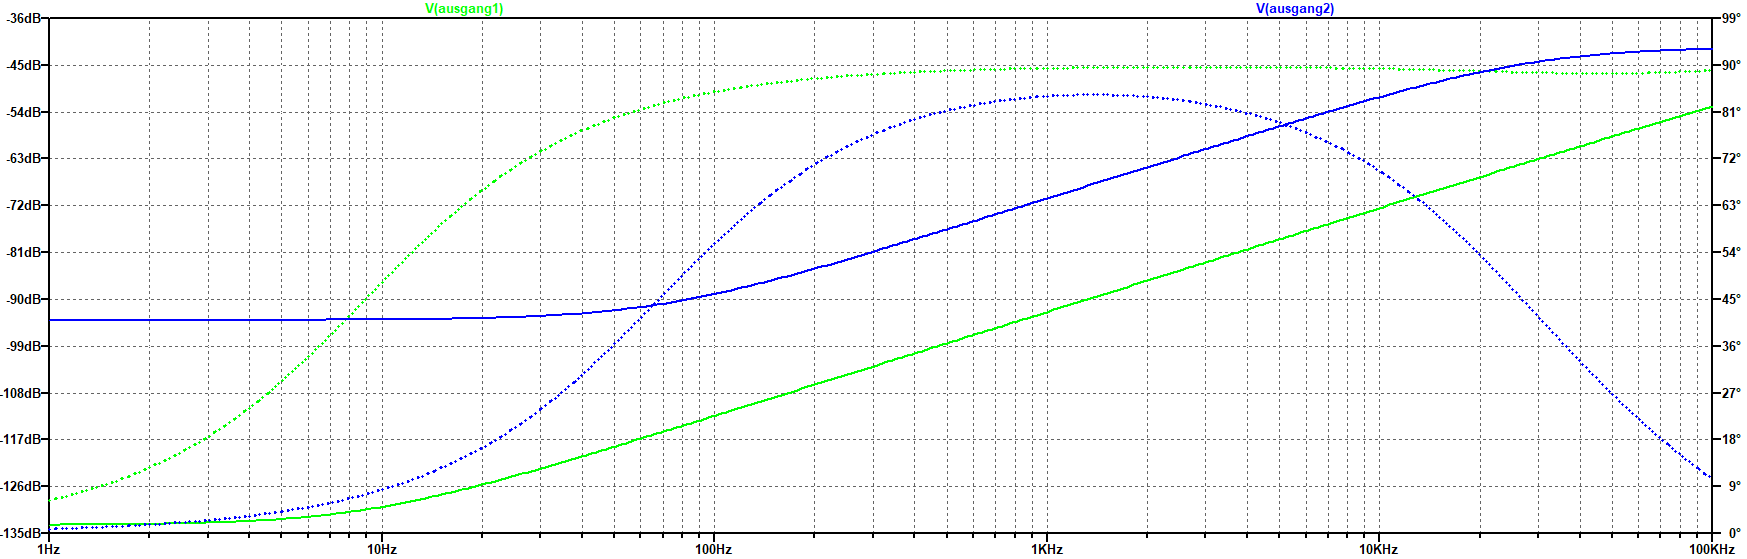
\includegraphics[width=\linewidth]{gleichtakt.png}
            \caption{Diagramm des Frequenzgangs Gleichtaktverstärkung}
        \end{figure}
        Bei einem Insturmentenverstärker liegt die niedrigste Gleichtaktfrequenz bei \(f=\SI{1}{\Hz}\). Mit hilfe der Curserfunktion wird nun die Verstärkung beider Ausgänge ausgelesen. 
        Für den Instrumentenverstärker aus drei Operationsverstärkern ergibt sich die niedrigste Gleichtaktverstärkung von \(v_{CM}=-\SI{133,371}{\dB}\) bei einer Frequenz von \(f=\SI{1}{\Hz}\)~\figref{gleichtaktwerte}.
        Für den integrierten Instrumentenverstärker ergibt sich die niedrigste Gleichtaktverstärkung von \(v_{CM}=-\SI{94,000}{\dB}\) bei einer Frequenz von \(f=\SI{1}{\Hz}\).
        Aus den Datenblätter lassen sich die Werte für die Gleichtaktunterdrückung \(v_{cmrr}\) entnehmen.
        \begin{table}[h!]
            \centering
            \caption{Ergebnisse der Gleichtaktverstärkung über den Frequenzgang}
            \begin{tabular}{|c|c|c|}
                \hline
                für \(f=\SI{1}{\Hz}\)  & Sim. \(v_{CM}\) & \(v_{cmrr}\) der Datenblätter\\ \hline 
                TL084 & \(\SI{-133,371}{\dB}\)&\(\SI{86}{\dB}\)\\ \hline
                AD8226 & \SI{-94,000}{\dB}&\(\SI{120}{\dB}\)\\ \hline
            \end{tabular}
        \end{table}
        Der Instrumentenverstärker aus drei Operationsverstärkern hat eine geringe Gleichtaktverstärkung bei \(f=\SI{1}{\Hz}\), dieser Wert ist deutlich niedriger als der Wert aus dem Datenblatt. Ursache hierfür ist die Tatsache das mehrere Operationsverstärker vom Typ TL084 verbaut sind. 
        Hinzu zufügen ist das der Wert \(v_{cmrr}=\SI{86}{\dB}\) kein maximal Wert ist.\par
        Der integrierte Instrumentenverstärker liefert laut Datenblatt eine Gleichtaktunterdrückung von minimal \(v_{cmrr}=\SI{120}{\dB}\) und bei Frequenzen \(f>\SI{5}{\Hz}\) eine Unterdrückung von \(v_{cmrr}=\SI{90}{\dB}\). Dies stimmt mit der Simulation nur bedingt überein. \par
        Bei beiden Integrationsverstärker sieht man mit zunehmender Frequenz eine stetig wachsende Verstärkung. Der Grund hierfür liegt daran, dass reelle Instrumentenverstärker simuliert werden und diese in ihren Operationsverstärkern zum Eingang eine parallel geschaltete parasitäre Kapazität besitzen. 
        Die hat eine negative Auswirkung auf die Gleichtaktunterdrückung, da sie mit steigender Frequenz zunehmend leitend wirken. 
        
        \begin{figure}[ht!]
            \centering
            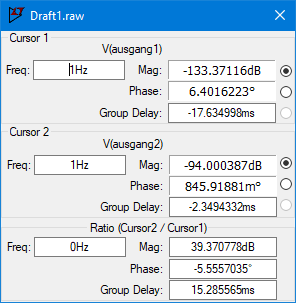
\includegraphics[]{gleichtaktwert.PNG}
            \caption{Gleichtaktverstärkung von Ausgang 1 und 2}
            \label{gleichtaktwerte}
        \end{figure}
        \newpage
    \section{Einfluss von Widerstandstoleranzen}
        Um den Einfluss zu messen, den ein Widerstand mit einer Toleranz von \(\pm \SI{1}{\ohm}\) hat, wird der Wert von \(R_6\) um \SI{1}{\percent} gesenkt.
        Hierbei ergibt sich ein neuer Wert für von \(R_6= \SI{33}{\kilo\ohm}\cdot 0,99 = \SI{32,670}{\kilo\ohm}\). Die Simulation wird mit dem abgeänderten Wert von \(R_6\) durchgeführt. Am \textbf{Ausgang 1} kann man folgenden Graf ablesen.
        \begin{figure}[ht!]
            \centering
            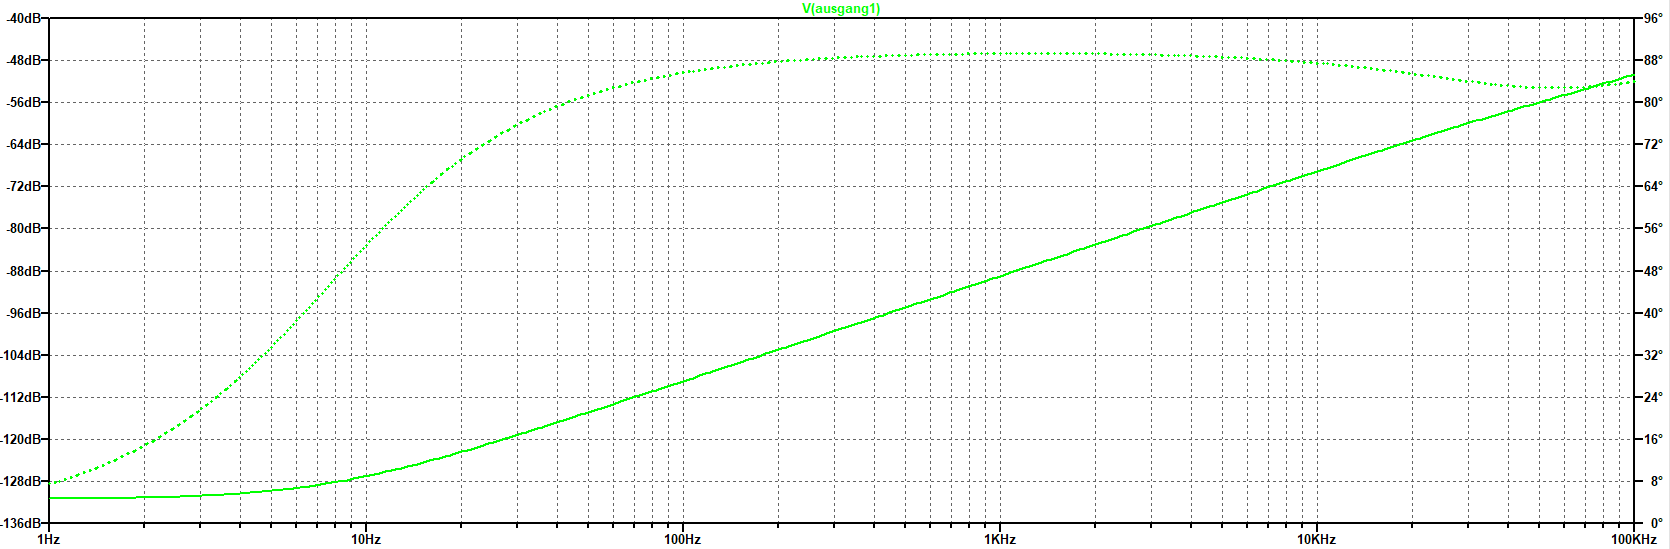
\includegraphics[width=\linewidth]{widerstandr6.PNG}
            \caption{Graf der Schaltung mit verändertem R6}
        \end{figure}
        Auch hier wird mit hilfe der Curserfunktion der Wert \(f=\SI{1}{\Hz}\) abgelesen. Hier kann man ein Wert von \(v_{tol1} = -\SI{133,237}{\dB}\) sehen. \par
        Um die Auswirkung einer Toleranz von \SI{1}{\percent} zu sehen werden alle Werte der Widerstände 1-7 um die Toleranz geändert~\figref{toleranzschaltung}. 
        \begin{figure}
            \centering
            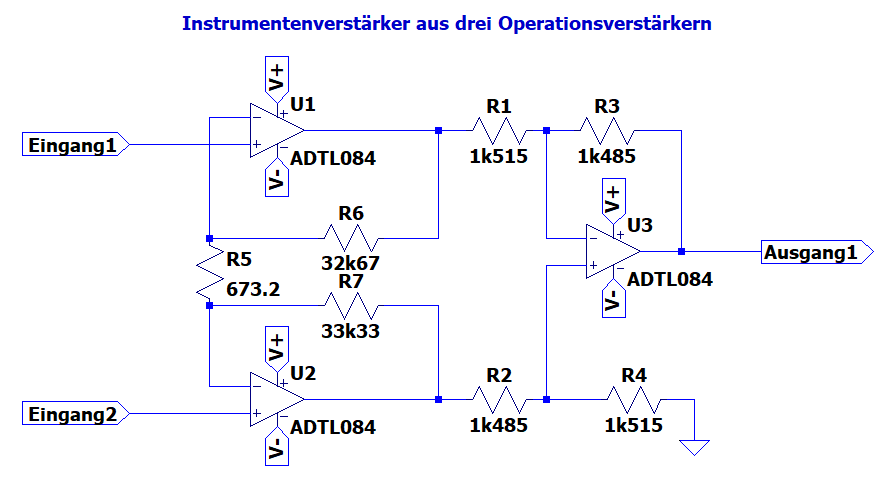
\includegraphics[width=\linewidth]{maxtoleranz.PNG}
            \caption{Schaltung mit allen Widerständen um \(\pm\SI{1}{\percent}\) geändert}
            \label{toleranzschaltung}
        \end{figure}
        Wird nun die Simulation gestartet erhält man den Frequenzgang aus ~\ref{toleranzgraf}.
        \begin{figure}[ht!]
            \centering
            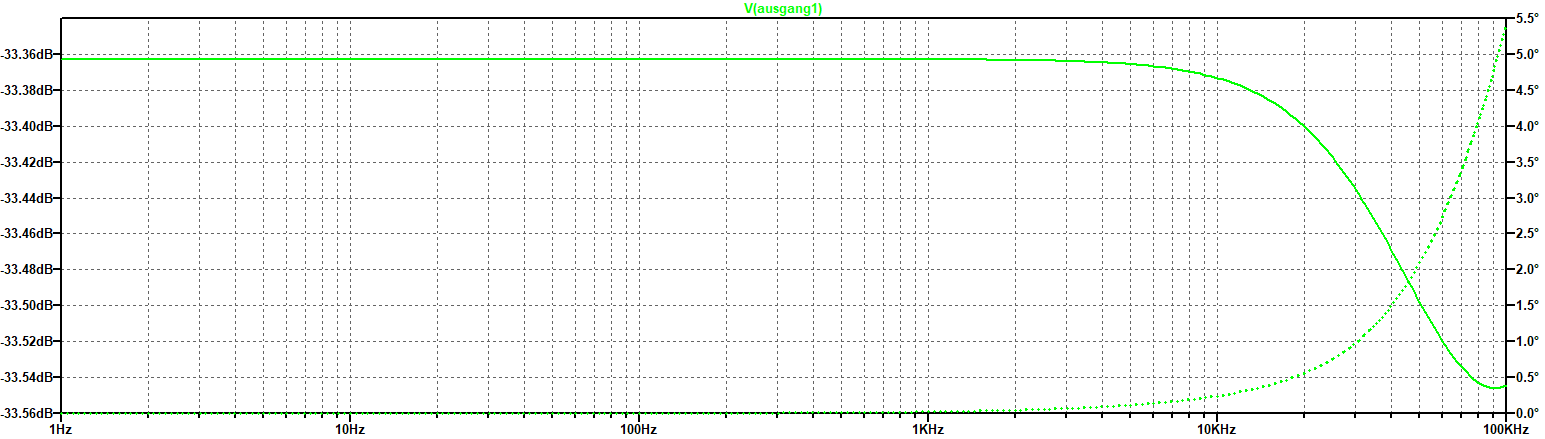
\includegraphics[width=\linewidth]{toleranzwerte.PNG}
            \caption{Gleichtaktverstärkung mit veränderten Widerstandstoleranzen}
            \label{toleranzgraf}
        \end{figure}

        \begin{table}[h!]
            \centering
            \caption{Ergebnisse der Gleichtaktverstärkung über den Frequenzgang}
            \begin{tabular}{|c|c|c|c|}
                \hline
                für \(f=\SI{1}{\Hz}\)  & indeale Widerstände & \(R_6\) mit Toleranz der Datenblätter & alle R mit Toleranz\\ \hline 
                \(v_{CM}\) in dB & \(\SI{-133,371}{\dB}\)&\(-\SI{133,237}{\dB}\)&\(-\SI{33,363}{\dB}\)\\ \hline
            \end{tabular}
        \end{table}
        Hierbei zeigt sich das wenn nur ein Wiederstand (\(R_6\)) vom Idealwert abweicht, die Veränderung quasi Null ist. Auch wenn man andere Widerstände einzeln verändert, wirkt es sich quasi garnicht auf die Verstärkung aus. 
        Werden alle Widerstände jedoch verändert, hat dies große Auswirkungen auf die Gleichtaktunterdrückung. Diese steigt stark an und damit sinkt die Gleichtaktverstärkung. 

        %\chapter{Auswertung der Berechnung und Simulation}
    \section{Spannung in den Arbeitspunkten}
        Der Unterschied in Tab~\ref{tab:arbeit} zwischen den berechneten und simulierten Werte sind geringfügig und zeigen dass, die Simulation akkurat arbeitet. 
        \begin{table}[h!]
            \centering
            \caption{Table to test captions and labels}
            \begin{tabular}{| c | c | c | c |} 
                \hline
                & \(U_A\) in \SI{}{\V} & \(U_B\) in \SI{}{\V}  & \(U_C\) in \SI{}{\V}  \\
                \hline
                Berechnung & 2,609 & 1,347 & 13,88 \\ 
                \hline
                LTSpice & 2,557 & 1,332 & 13,968 \\
                \hline
            \end{tabular}
            \label{tab:arbeit}
        \end{table}
    \section{Ein-und Ausgangswiderstand}
        Der Unterschied in Tab~\ref{tab:widerstand} zwischen den berechneten und simulierten Werten des \(R_{ein}\) weichen um \SI{2.441}{\kilo\ohm} ab. Diese Abweichung kann Resultat dessen sein dass, die Stromverstärkung \(\beta\) mit einem Wert von 300 angenommen wird.
                \begin{table}[h!]
            \centering
            \caption{Table to test captions and labels}
            \begin{tabular}{| c | c | c |} 
                \hline
                & \(R_{ein}\) in \SI{}{\kilo\ohm} & \(R_{aus}\) in \SI{}{\kilo\ohm}    \\
                \hline
                Berechnung & 26,25 & 10 \\ 
                \hline
                LTSpice & 28,696 & 10  \\
                \hline
            \end{tabular}
            \label{tab:widerstand}
        \end{table}
    \section{Spannungsverstärkung und Frequenzganganalyse}
        Die Werte in Tab~\ref{tab:frequenz} der Grenzfrequenz passen genau zu einander. Der Unterschied bei der Spannungsverstärkung  beläuft sich auf einen Wert von \(\Delta = \SI{0.434}{\dB}\).
        \begin{table}[h!]
            \centering
            \caption{Table to test captions and labels}
            \begin{tabular}{| c | c | c | c |} 
                \hline
                & \(\upsilon_{dB}\) in \SI{}{\decibel} & \(f_u\) in \SI{}{\Hz}  & \(f_o\) in \SI{}{\Hz}  \\
                \hline
                Berechnung & 20 & 60,630 & 72,340 \\ 
                \hline
                LTSpice & 19,566 & 60,729 & 13,968 \\
                \hline
            \end{tabular}
            \label{tab:frequenz}
        \end{table}
    \section{Temperaturabhängigkeit des Arbeitspunktes C}
        Alle simulierte Werte in Tab~\ref{tab:temp} sind ca. um \(\Delta U_C\approx \SI{100}{\milli\volt}\) größer als die berechneten Werte.
        \begin{table}[h!]
            \centering
            \caption{Table to test captions and labels}
            \begin{tabular}{| c | c | c | c |} 
                \hline
                & \(U_C\) bei \SI{0}{\degreeCelsius} & \(U_C\) in \SI{25}{\degreeCelsius}  & \(U_C\) in \SI{100}{\degreeCelsius}  \\
                \hline
                Berechnung & 14,034 & 13,88 & 13,409 \\ 
                \hline
                LTSpice & 14,123 & 13,979 & 13,543 \\
                \hline
            \end{tabular}
            \label{tab:temp}
        \end{table}
        %\chapter{Fazit}
Bei dem Versuch werden erstmal die Grundlegenden Begriffe der Gleich- und Wechselspannung erklärt. 
Diese sind dann durch ein Voltmeter in die Schaltungen eingebracht worden. 
Dabei sind Schaltungen wie der Spannungsteiler und das Potentiometer aufgebaut worden 
und durch LTSpice simuliert. Zum besseren Verständnis des Graphen wurde 
dann der Effektivwert sowie die Ausgangsspannung per Hand ausgerechnet und mit den von 
LTSpice simulierten Werten verglichen. Die Werte für den Spannungsteiler und den Potentiometer
 haben mit den zu erwarteten Werten wunderbar funktioniert. Bei dem Rechtecksignal einer 
 Spannungsquelle sind jedoch zwischen simuliertem und berechneten Effektivwert Differenzen 
 aufgetreten. Ursprung des Fehlers kann in der Rechnung liegen, obwohl diese öfters zum Überprüfen 
 der Richtigkeit durchgeführt wurde. Der Fehler kann auch in der falschen Durchführung von 
 LTSpice liegen. In der Aufgabenstellung von 2.1 (Signalquellen), war nicht genau ersichtlich ob 
 das Voltmeter durch eine Wechselspannung oder Gleichspannung angetrieben wird. Durch eine 
 Wechselspannung würde der Graph von -1V bis 1V gehen. Die simulierten Graphen in dem Bericht 
 sind jedoch nur von 0V bis 1V aufgetragen. Durch die Wechselspannung sind die berechneten Werte 
 aber auch nicht zu erzielen, da diese ebenfalls zur Lösung des Problems simuliert wurden und 
 nicht mit den berechneten Werten übereinstimmen. 
         %\chapter{Quellen}
\section*{Bilder}
\textbf{[B~\ref{fig:242}] und [B~\ref{fig:252}]}     https://www.onsemi.com/pub/Collateral/BC550-D.pdf\\
(18:03/10.01.2021)
    
    
    \printbibliography
\end{document}